\chapter{Grundlagen}
    Übergangsmetalloxide zeigen zahlreiche und unterschiedlichdte Eigenschaften.
    Ihre große Varriation ist Thema aktueller Forschung und soll im \autoref{sec:TMO} genauer behandelt werden.
    Eine besondere Untergruppe der Übergangsmetalloxide sind die Antiferromagneten.
    Durch die antiferromagnetische Kopplung der Lagen ergeben sich neue Phänomene, wie eine hohe Magnonenfrequenz.
    Auf diese Materialeigenschaft soll in \autoref{sec:AFM} eingegangen werden.
    Organisch-inorganische-Grenzflächen find heute bereits Anwendung in organischen Leuchtdioden und organischen Feldeffekttransistoren.
    Hierfür ist die Wechselwirkung der oranischen Materialien mit den inorganischen Oberflächen relevant.
    Genaueres hierzu findet sich in \autoref{sec:WW}.
    In dieser Arbeit werden verschiedene Substarte und Oberflächenorientierungen verwendet um das Verhalten von Pentacene Molekülen auf den antiferromagnetischen Oberflächen zu untersuchen.
    Eine Einführung und Überblick über die verwendeten Systeme wird in \autoref{sec:Systeme} gegeben.
    
    % In diesem Kapitel wird eine Einführung in die Grundlegenden Eigenschaften der untersuchten Systeme gegeben.
    % Zunächst geht es um die Materialklasse der Übergangsmetalloxide, da dies in der vorliegenden Arbeit genauer untersucht werden.
    % Anschließend geht es um den Antiferromagnetismus, welcher die magnetischen Strukturen innerhalb der Proben beschreibt.
    % Dann geht es um die Wechselwirkung zwischen Oberflächen und Molekülne und wie diese sich auf der Oberfläche bezüglich ihrer geometrischen und elektronischen Struktur verändern.
    % Zuletzt werden dann die Oberflächen und Moleküle eingeführt, welche zur Präperation der verwendeten Proben genutzt wurden.

    \section{Übergangsmetalloxide} \label{sec:TMO}
        Übergangsmetalloxide finden sich in einer Vielzahl in unserer Umwelt, meist jedoch unter anderem Namen.
        So ist der Rost wohl eins der Bekanntesten, dabei handelt es sich um eine Form des Eisenoxids.
        Magnetit hingegen ist in der Wissenschaft sehr bekannt, da es das ersten entdecken magnetischen Material ist~\cite{Magnetit}.
        Die Eigenschaften der Übergangsmetalloxide varrieren in einem sehr großen Bereich.
        So gibt es ferro- und antiferromagnetische Übergangsmetalloxide.
        Die elektrische Leitfähigkeit varriert dabei von leitende, sogar Hochtemperatur supraleitende über halbmetallisch bis hinzu isolierend~\cite{IF_5}.
        Durch ihrer Anpassbarkeit und einfache Herstellung sind sie damit ideale Kandidaten für Anwendungen.
        Hierdurch sind die Übergangsmetalloxide in den letzten Jahren auch immer mehr in den Fokus der aktuellen Forschung geraten~\cite{IF_6, parkinson_iron_2016, cornell_iron_2003}.
        Anwendung finden sie schon heute zum Beispiel in organischen Transistoren, Solarzellen und LEDs~\cite{IF_3}.
        Oder im Fall des Magentits in Magnetstreifen.

        Übergangsmetalloxide bestehen aus einem Übergangsmetall, dem Kation und Sauerstoffatomen als Anion.
        Bei der Bindung zwischen dem Sauerstoff und dem Übergangsmetall sind dessen p-Orbitale, sowie die s-Orbitale des Metalls beteiligt.
        Dies führt zu eine Hybridisierung und Ausbildung neuer Zustände.
        Ferner fallen die s-Orbital Elektronen als Ladungsabschirmung bei den d-Elektronen des Übergangsmetalls weg.
        Hierbei kommt es zur starken Elektron-Elektron-Wechselwirkung unter den d-Elektronen, diese Korrelation sorgt für eine starke Lokalisierung~\cite{dane_beschreibung_2008}.
        In Anwesenheit des Kristallfeldes der Liganden spalten die entarteten Zustände auf.
        Bei Monooxiden, wie dem Nickeloxid (\ce{NiO}) und Wüstit (\ce{FeO}) nehmen die Übergangsmetallionen eine oktaedrisch Position zwischen den Sauerstoffionen ein.
        Wodurch die Orbitale $d_{z^2}$ und $d_{x^2-y^2}$ energetisch angehoben und die anderen energetisch abgesenkt werden.
        Die so entstandenen neuen Energieniveaus lassen durch die Wechselwirkung zwischen Ladung, Orbitalen, Gitter und Spin auch magnetische Eigenschaften aufleben.
        So können sich durch die Kristallfeldaufspaltung \textit{High}- und \textit{Low}-Spin Konfigurationen ausbilden.
        Die Eigenschaften werden maßgeblich durch den Überlapp der beteiligten Orbitale bestimmt~\cite{kupper_electronic_2005}.
        In Folge dessen sind sie abhängig von den Oxidationszuständen, der Stochimetrie und der Struktur.

        \begin{figure}
            \centering
            \begin{subfigure}{0.48\textwidth}
                \centering
                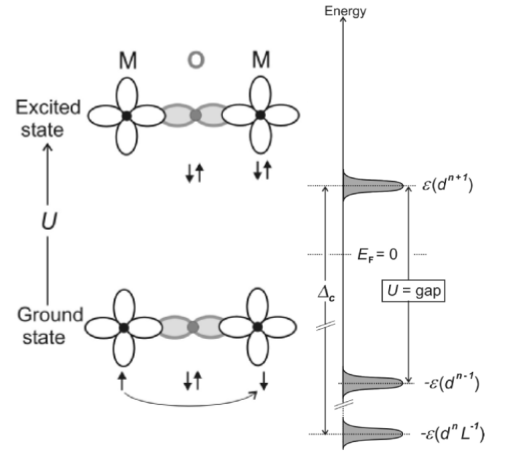
\includegraphics[height=5cm]{Mott_mod.PNG}
                \subcaption{}
                \label{fig:Mott}
            \end{subfigure}
            \begin{subfigure}{0.48\textwidth}
                \centering
                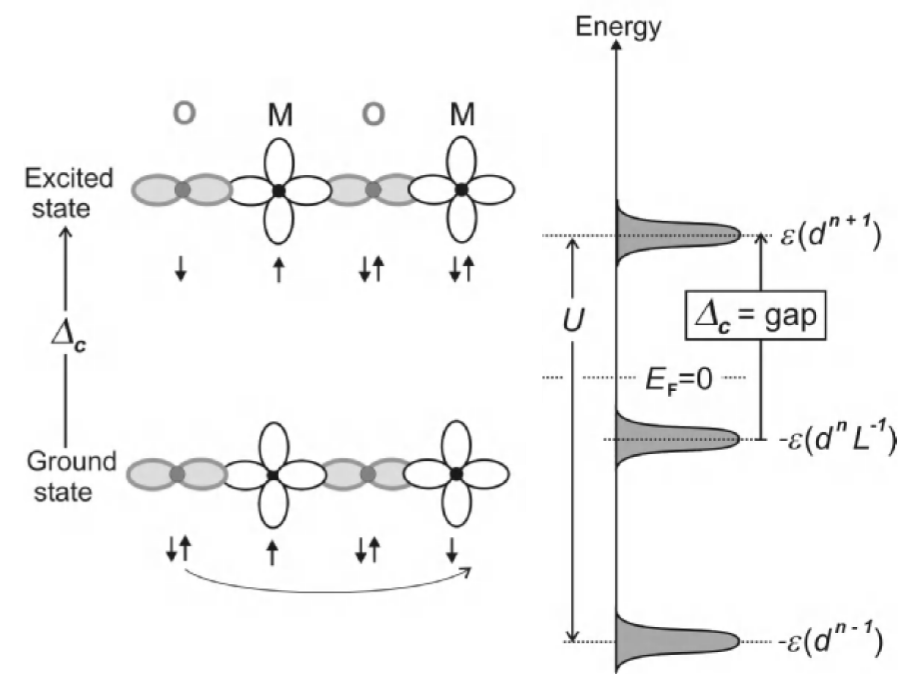
\includegraphics[height=5cm]{Charge_mod.PNG}
                \subcaption{}
                \label{fig:Charge}
            \end{subfigure}
            \caption{Veranschaulichung des Mott-Hubbard-Isolators (\subref{fig:Mott}) und des Ladungs-Transferisolators (\subref{fig:Charge}).
            Dabei befindet sich links im Bild stets die Abbildung im Realraum, wohingegen rechts die Abbildung im raum der Zustandsdichte dargestellt ist.
            Entnommen und modifiziert aus~\cite{stohr_magnetism_2006}.}
            \label{fig:Bandl}
        \end{figure}
        Die Bandstruktur des Kristalls wird im niederenergetischen Valenzbandbereich durch die überlappenden 2p-Orbitale des Sauerstoffs dominiert.
        Zu höheren Energien hin rührt die Bandstruktur von den überlappenden d-Orbitalen der Übergangsmetalle her.
        Dabei sind die 2p-Zustände stark besetzt wohingegen die d-Zustände nur schwach besetzt werden.
        Bei der Betrachtung der Bandstruktur der Übergangsmetalloxide ist zu beachten, dass diese eine Bandlücke zwischen Valenz- und Leitungsband aufweisen.
        Diese Bandlücke liegt dabei zwischen den besetzen Sauerstoffzuständen und den unbesetzten d-Zuständen des Übergangsmetall.
        Folglich handelt es sich also um Halbleiter oder Isolatoren.

        Es können sich zwei Arten von Bandlücken ausbilden, welche in \autoref{fig:Bandl} abgebildet sind.
        Wichtig hierfür ist die Austauschwechselwirkungsenergie $U$, welche die Energie darstellt um ein Elektron von einem Metallatom zu entfernen und es einem weiteren Metallatom hinzuzufügen.
        Auch die Ladungsübertragsenergie~$\Delta$ ist zur Beschreibung notwendig, diese stellt die Energie da, um ein Elektron aus dem Liganden zum Metall zu übertragen~\cite{stohr_magnetism_2006}.
        Die erste Art der Bandlücke ist die in der $U$ größer ist als $\Delta$, hierbei handelt es sich um Mott-Hubbard-Isolatoren und die Bandlücke wird durch $U$ definiert.
        Im Gegensatz dazu, wenn $\Delta < U$ handelt es sich um so gennate Ladungstransfer-Isolatoren und die Bandlücke wird durch $\Delta$ beschrieben.
        Zu diesen zählt das Nickeloxid und Wüstit, dass trotz teilweise gefüllten d-Bändern Isolatoren sind~\cite{IF_5}.

        Im Gegensatz zu kristallienen Eigenschaften sind die Eigenschaften von dünnen Filmen und Oberflächen noch wenig erforscht.
        Dünne Filme aus Übergangsmetalloxiden stellen einen Teilbereich dar und bringen durch ihre zusätzlichen Einschränkung neue Möglichkeiten mit.
        So lässt sich im Fall von Eisenoxid ein dünner Film von Magnetit (\ce{Fe3O4}) durch heizen in Wüstit (\ce{FeO}) überführen~\cite{FeO_1}.
        Durch Ionen induziertes Zerstäuben lässt sich aus Hämatit (\ce{Fe2O3}) ebenfalls Wüstit gewinnen~\cite{FeO_36}.
        Die chemischen und elektrochemischen Eigenschaften der Filme hängen also maßgeblich vom Präperationsprozesse ab und können zu unterschiedlichen Ergebnissen und damit Eigenschaften führen~\cite{Uni-Tübingen}.
        Durch gezieltes Eingreifen in den Präperationsprozess, z.B. Variation aus dem Verhältnis des Sauerstoffdrucks zur Aufdampfrate lässt sich die Stochimetrie varrieren.
        Alleine durch die Veränderung des Oxidationszustands oder Einbringen von Defekten lässt sich die Austrittsarbeit der Oxide anpassen.
        Diese ist ein entscheidener Parameter bei der Energieniveauanpassung zwischen Substrat und Molekülen, infolge dessen es zu einem einfachen Ladungstransfer kommen kann~\cite{IF_3}.
        Genaueres hierzu wird in \autoref{sec:ENA} behandelt.

        Wichtig für die Interaktion mit Adsorbaten ist die Grenzfläche.
        An der Oberfläche spielen die Polarität, Anzahl ungesättigter Bindungen wie auch Defekte eine entscheidene Rolle bei der Oberflächenrekonstruktion und Reaktivität.
        Die hier untersuchten Monooxid Systeme, mit der Beteiligung von 3d-Übergangsmetallen kristallisieren in der Kochsalzstruktur.
        % Im Gegensatz dazu kristallisiert das Magnetit (\ce{Fe3O4}) in der inversen Spinellstruktur~\cite{IF_5}.
        Die Oberflächen der Kochsalzstruktur mit der (100)-Orientierung sind meist stabil, wohingegen die der (111)-Orientierung instabil sind.
        Dies liegt an der polaren Oberfläche der (111)-Orientierung und des damit verbundenen großen Oberflächendipolmoments.
        Hierdurch wird eine größere Reaktivität der Oberfläche erwartet~\cite{cappus_hydroxyl_1993}.
        % Anzumerken bleibt, dass dabei die Sauerstoff terminierte Oberfläche stabiler als die metallisch terminierte Oberfläche ist.
        % Ursache ist die einfachere Polarisation des Sauerstoffatoms, was das Oberflächendipolmoment reduzieren kann~\cite{al-abadleh_oxide_2003}.
        Solche reaktiven Oberflächen, meist aus dünnen Filmen werden heute bereits zur Katalyse eingesetzt.

        \begin{itemize}
            \item Oberflächen und Grenzflächen zeigen neue Eigenschaften und Phasen -> Anwendung 
            \item Symmetriebrechung, Verspannung (WW mit Substrat), Polarität, Filmdicke, Kristallograpische Orientierung
            \item Die starke Wechselwirkung der e ist die Ursache für die zahlreichen effekte wie Supraleitung und magnetisms in TMO 
            \item Verständnis ist wichtig um Phasenübergänge durch gezielten Doping, Temperatur oder äußeres Magnetfeld für die Anwendung nutzbar zu machen
            \item Magnetische Widerstandsänderung erläutern? (GMR, TMR, CMR)
            \item Anpassung der Austrittsarbeit bei der Anwendung, damit Kontaktwiderstand minimiert wird zwischen inorganischer Schicht und Elektrode \cite{IF_11, NiO_40}
            \item Vor allem in dem \ce{Fe3O4} in dem das Eisen als (2+) und (3+) Ion auf unterschiedlichen Gitterplätzen (tetraedisch oder oktaedrisch) vorkommt, kommt es zu unterschiedlichen Aufspaltungen der $e_g$ und $t_{2g}$ Energieniveaus.
        \end{itemize}

    
    \section{Antiferromagneten} \label{sec:AFM}
        Antiferromagneten (AFM) zeichnen sich dadurch aus, dass Sie nach außen hin kein permanetes magnetisches Moment aufweisen.
        Vereinfacht sind im Inneren die magnetischen Momente vom gleichen Betrag und nebeneinander liegende Momente sind antiparallel untereinander ausgerichtet~\cite{Suter}.
        Dieser Zustand ist allerdings nur unterhalb der Néel-Temperatur $T_\text{N}$ stabil, oberhalb verhälten sich die Antiferromagneten paramagnetisch.
        Die inneren magnetischen Momente richten sich dabei parallel zum äußeren Feld aus und verstärken es somit.
        Um das Phänomen des Antiferromagnetismus zu erklären Bedarf der quantenmechanischen Beschreibung unter Beachtung des Pauli Verbots und der Hundschen Regeln~\cite{TUChemnitz}.
        Es ergibt sich der Austauschwechselwirkungshamiltonien $H_\text{A} = - J_{ik} \vec{S_i}\cdot\vec{S_k}$ der die direkte Wechselwirkung der Spins berücksichtigt.
        Für $J_{ik} < 0$ ergibt sich die antiferromagnetische Kopplung und für $J_{ik} > 0$ eine ferromagnetische Kopplung.
        $J_{ik}$ spiegelt dabei die Stärke der Austauschwechselwirkung wieder und folgt aus dem Überlapp der Wellenfunktionen der beteiligten Elektronen.
        Um eine Aussage über die Ordnung im Antiferromagnet zutreffen gibt es den Ordnungsparameter $L = S^{\uparrow} - S^{\downarrow}$.
        Hierbei ist $S^{\uparrow}$ beziehungsweise $S^{\downarrow}$ der Spin der jeweiligen Untergitter.

        \begin{figure}
            \centering
            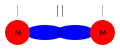
\includegraphics[width=0.6\textwidth]{AFM2.pdf}
            \caption{Darstellung zur Veranschaulichung der antiferromagnetischen Kopplung.
            Als Ligand fungiert hier ein Sauerstoffatom mit seinem p-Orbital (blau).
            Die Spins der d-Orbitale der Metalle (rot) koppeln ferromagnetische mit denen des Sauerstoffs.
            So entsteht die antiferromagnetische Kopplung der beiden Metallatome.}
            \label{fig:AFM}
        \end{figure}
        Ursache des Antiferromagnetismus ist der Superaustausch.
        Beim Superaustausch koppeln zwei Atome mit einem magnetischen Moment über ein weiteres nicht magnetische Atom. 
        Dabei kann die Kopplung ferro- oder antiferromagnetisch sein, meist jedoch antiferromagnetisch~\cite{AFM_1}.
        Sind die beiden koppelnden magnetischen Momente nicht gleich groß, so tritt Ferrimagnetismus auf, es gibt dann eine makroskopische Magnetisierung.
        Der Superaustausch ist winkelabhängig, da es dabei um den Überlapp der Orbitale geht.
        Für die Erklärung wird sich hier nur auf die \SI{180}{\degree} Wechselwirkung beschränkt.
        Beispielhaft ist die Kopplung in \autoref{fig:AFM} dargestellt.
        Es kommt bei diesem indirekten Austausch nicht zu einem Überlapp der spintragenden Wellenfunktionen sondern zu der Vermittlung der langreichweitigen Ordnung über einen Liganden.
        Direkter Austausch sorgt für ferromagnetische Kopplung benachbarter andersartiger (nicht magnetischer) Atome.
        Zwischen Metall und Ligand herscht also direkte Austauschwechselwirkung und damit eine indirekte Austauschwechselwirkung, der Superaustausch zum übernächsten Atom, einem weiteren Metallatom.
        Bei den vorliegenden Metalloxiden ist es so, dass die Elektronen der Metallatom des nicht vollen 3d-Oribtals über die 2p-Orbitale des Sauerstoffs koppeln.
        Da dieses Orbital voll ist, müssen die Elektronen unterschiedliche Spinrichtung haben.
        Damit besitzten die Sauerstoffatome auch kein eigenes magnetisches Moment.
        Somit ist die Wechselwirkung über das Sauerstoffatom hinweg antiferromagnetisch.
        Es ergeben sich zwei Untergitter, welche unterschiedlicher Spinrichtung sind, die Gesamtmagnetisierung ist wie für Antiferromagneten erwartet Null.
        % Die Wellenfunktionen der Kationen überlappen nur gering und da die Austauschwechselwirkung nur geringe Reichweiten hat können nur die 3d und 2p überlappen.
        
        Die Anwendungen des Antiferromagnetismus ist zum Beispiel der Nutzen als \textit{Pinning}-Lage, die in spinelektronischen Bauteilen die Orientierung einer ferromagnetischen Schicht festlegt.
        Eine neue Forschungsidee des europäischen Forschungsprojekt Sinfonia beschäftigt sich mit der Kopplung zwischen Molekülen und Antiferromagneten.
        Ferner sollen diese genutzt werden um Spinwellen, so genannte Magnonen zu generieren und zu detektieren.
        Dies könnte auf Grund der Magnonenfrequenz im \si{\tera\hertz}-Bereich neue Geschwindigkeitsrekorde in der Datenverabeitung bringen~\cite{SINFONIA}.
        In Folge dessen werden in dieser Arbeit erste Charakterisierungen für potenzielle Substrate und Moleküle untersucht.
                
    
    \section{Wechselwirkung von Oberfläche mit Molekülen} \label{sec:WW}
        Moleküle haben im Gegensatz zu Festkörpern, energetisch separierte Zustände, die Orbitale.
        Werden Molekül auf eine Oberfläche aufgebracht so kommt es zur Wechselwirkung zwischen diesen und der Struktur der Oberfläche.
        Bei der Wechselwirkung von Molekülen mit Oberflächen wird in zwei Arten der Adsorption unterschieden. 
        Zum Einen in die der Physisorption und zum Anderen in die der Chemisorption, welche wiederum in stark und schwach unterschieden wird.
        Zwischen den beiden Adsorptionsarten lässt sich durch ihre Bindungsstärke zum Substrat hin unterscheiden.
        Dabei wird als Bindungsstärke die Energie bezeichnet, die nötig ist um ein Molekül von der Oberfläche zu lösen.
        In beiden Fällen handelt es sich um eine Adsorption die auch die Oberflächenstruktur des Substrates beeinflussen können.
        So können neue Zustände entstehen und vorhandene Eigenschaften stark verändert werden.
        %~\cite{ma-DJ
        
        \subsection{Physisorption}
            Der schwächste Adsorptionsprozess ist die Physisorption, bei der maßgeblich die Van-der-Waals-Kraft eine Rolle spielt.
            Sie hat dabei nur eine geringe Bindungsenergie der Moleküle zum Substrat~\cite{IF_16}.
            Da die Wechselwirkung bei der Physisorption nur gering ist werden die Eigenschaften der Oberfläche und des Moleküles nur schwach beeinflusst~\cite{bergenti_spinterface_2019}.
            Die Eigenschaften der Moleküle ähneln also sehr stark den Eigenschaften aus der Gasphase~\cite{IF_16}.
            Allerdings kann es beim Substrat zu Relaxation kommen.

            %, sowie einen Substrat-Adsorbat-Abstand von mehr als \SI{3}{\angstrom}. %~\cite{bergenti_spinterface_2019}
            % Die Van-der-Waals-Kraft kann man in drei Arten unterteilen:
            % \begin{itemize}
            %     \item \textbf{Dipol-Dipol-Kraft:} Sie ist die Kraft zwischen zwei permanenten Dipolen, die Keeson-Wechselwirkung.
            %     \item \textbf{Dipol-induzierter-Dipol-Kraft:} Die Wechselwirkung zwischen einem induziertem Dipol und einem Dipol wird auch als Debye-Wechselwirkung bezeichnet.
            %     \item \textbf{Londonsche Dispersions-Wechselwirkung:} Zwischen zwei induzierten Dipolen wirkt die Londonsche Dispersions-Wechselwirkung, sie dominiert meist die Van-der-Waals Kraft.
            % \end{itemize}

            Die Physisorption kann durch zwei Potetiale beschrieben werden.
            Das eine Potential wirkt repulsiv und resultiert aus dem Pauliverbot.
            Kommen sich Molekülorbital und Substratorbital zunah, überlappen diese.
            Auf Grund des Pauliverbots dürfen keine zwei Elektronen dann in allen Quantenzahlen übereinstimmen und es resultiert in eine abstoßende Kraft.
            Das zweite und attraktives Potentential resultiert dabei aus der Debye-Wechselwirkung.
            So kommt es beim Gleichgewicht zu einem stabilen Substrat-Molekül-Abstand.
            Das Gesamtpotential ist auch als Lennard-Jones-Potential bekannt.
            
            Die Van-der-Waals-Kraft gehört zu den elektrostatischen Kräften, es werden also keine Elektronen mit dem Substrat ausgetauscht~\cite{bergenti_spinterface_2019}.
            Allein die Induzierung und Fluktuation von Dipolen führt zu dieser Bindung zwischen Molekül und Substrat.
            Vermehrt tritt die Physisorption bei Halbleitern und Isolatoren auf, da die Molekülzustände in der Bandlücke liegen und so keine Bindung mit dem Substrat eingegangen werden kann~\cite{IF_1}.
            Charakteristisch für die Physisorption ist die Abwesenheit von chemischen Bindungen.
        
        \subsection{Chemisorption}
            % Im Gegensatz zur Physisorption findet bei der Chemisorption  ein Austausch von Elektronen stattfinden.
            Im Gegensatz zur Physisorption sind die Bindungen um Einiges stärker und führen somit zu Veränderung am Substrat wie auch den Molekülen~\cite{bergenti_spinterface_2019}.
            Ferner wird von Chemisorption gesprochen, wenn die Stärke der Wechselwirkung größer als \SI{1}{\electronvolt} ist~\cite{muscat_chemisorption_1978}.
            Aber dies allein ist nicht ausschlaggebend, es muss eine chemische Veränderung auftreten.
            Dabei kann es sich um kovalente und ionische Bindungen handeln und es kann zum Ladungsaustausch und/oder Hybridisierung kommen~\cite{harutyunyan_hybridisation_2013}.
            Beim Ladungsaustausch kann ein zunächst unbesetztes Orbital unter die Fermikante rutschen und besetzt werden, es kann also neben den strukturellen auch zu elektronischen Veränderungen kommen.
            Im Gegensatz dazu können bei der Hybridisierung mehrer Zustände vom Molekül und/oder Oberfläche durchmischt werden.
            Verbreiterungen, Verschiebungen und auch Aufspaltungen von Molekülzuständen kann die Folge sein~\cite{IF_1}.

            \begin{figure}
                \centering
                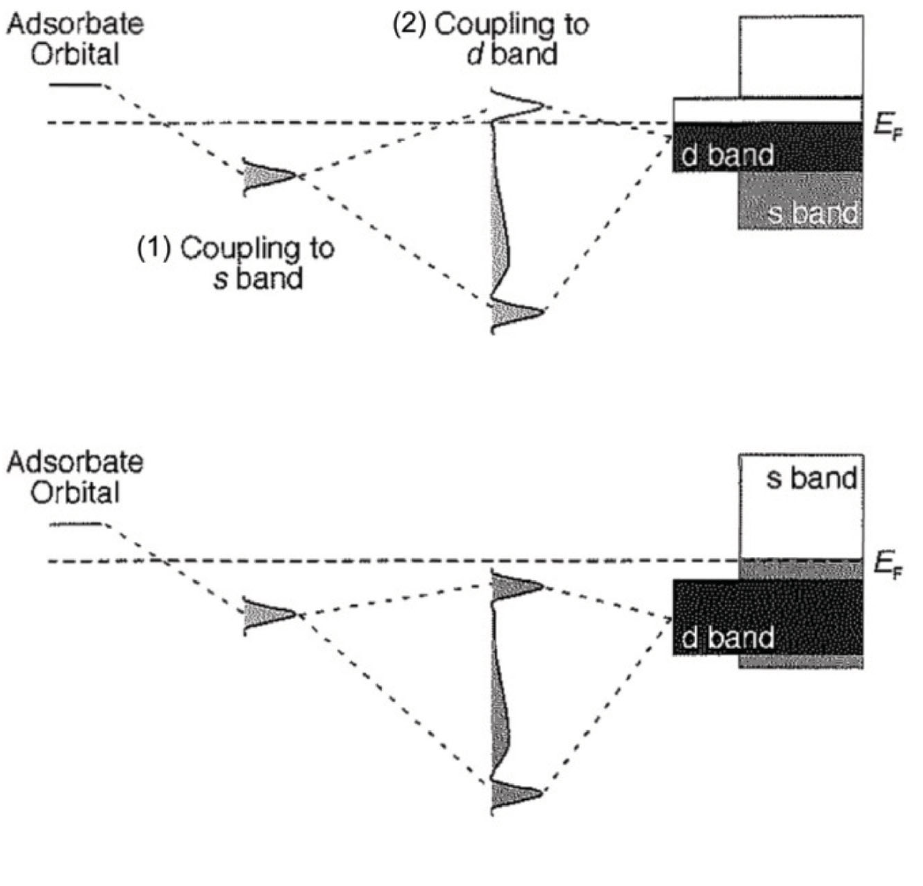
\includegraphics[width=0.5\textwidth]{Chemisorption2.PNG}
                \caption{Das adsorbierte Molekül hybridiziert mit dem s-/p-Band des Substrates (1), der schwachen Chemisorption.
                In einem weiteren Schritt kommt es dann zur starken Chemisorption durch Einbindung der d-Bänder (2, oben), es entsteht ein bindendes und ein antibindenes Orbital.
                Durch die Lage der d-Bänder werden nun das bindenden und antibindendene Orbital besetzt, dadurch kommt es zu einer repulsiven Kraft und die Bindung wird wieder geschwächt (unten). Aus~\cite{IF_1}.}
                \label{fig:Chemisorption}
            \end{figure}
            Schwache Bindungen werden meist durch die Wechselwirkung mit den breiten s- oder p-Bändern hervorgerufen.
            Wodurch sich das Energieniveau der Moleküle absenkt und verbreitert, siehe dazu in \autoref{fig:Chemisorption}.
            Für die starke Chemisorption folgt ein weiterer Schritt, der nun abgesenkte Zustand überlappt mit dem der näherungsweise d-Bänder.
            Es bilden sich bindende und antibindendene Zustände aus.
            Ja nach Lage des Ferminiveaus wird nur der bindende Zustand (starke Adsorption) oder auch (nur teilweise) der antibindende Zustand gefüllt.
            Durch die (teilweise) Füllung des antibindenden Zustands treten repulsiv Kräfte auf und die Adsorptionsstärke wird geschwächt.
            Ferner beeinflusst auch die Ausdehnung der d-Bänder die Stärke der Chemisorption.
        
        \subsection{Selbstanordnung} \label{sec:Selbstanordnung}
            Einige Moleküle ordnen sich regelmäßig auf einem Substrat an, dieser Effekt wird Selbstanordnung genannt.
            Dabei bilden die Moleküle eine Überstruktur im Vergleich zum Gitter des Substrates.
            Gewünscht ist dies, da dann die Molekül einheitlich auf der Oberfläche orientiert sind und somit auch ihre Orbitale, dies ist notwendig für die Molekülorbital-Tomographie (s. \autoref{sec:MOT}).
            Ferner lassen sich gitterartig verteilte Moleküle gezielter manipulieren, wie es für Anwendungen notwendig ist.
            
            \begin{figure}
                \centering
                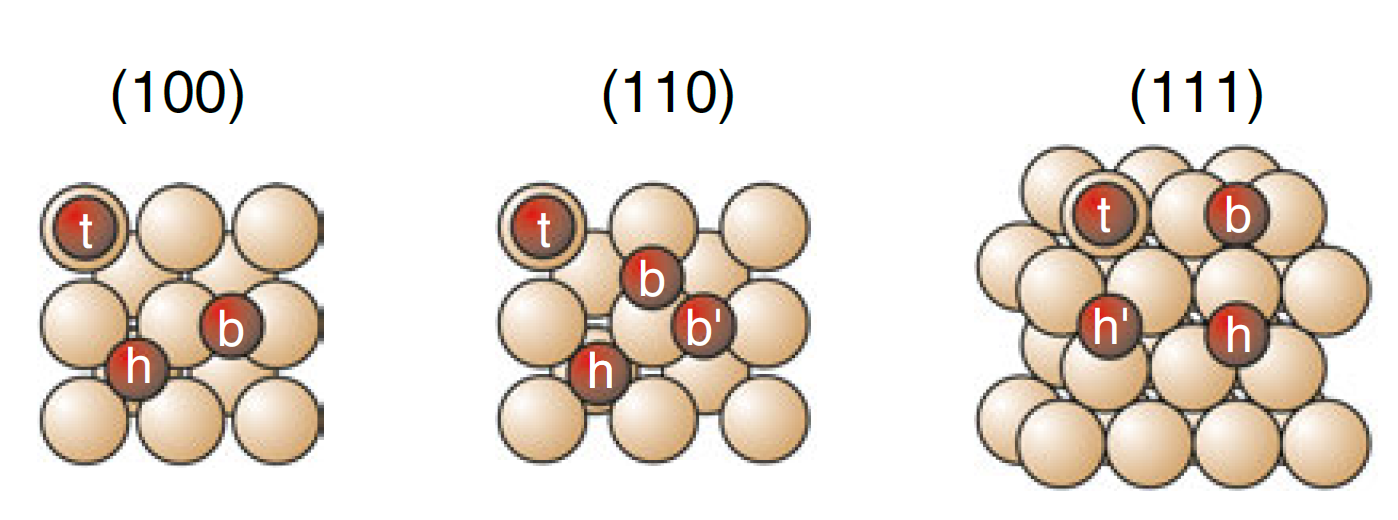
\includegraphics[width=0.6\textwidth]{Adsorbate}
                \caption{Die Adsorbateplätze für verschieden orientierte Oberflächen eines flächenzentrierten Kristalls.
                Es gibt Plätze direkt oberhalb eines Substratatoms (\textit{on top} - t).
                Zwischen zwei Substratatomen gibt es kurze (b) und lange (b') Brückenplätze (\textit{bridge}), sowie Muldenplätze hexagonaler dicht gepacktester Struktur (\textit{hollow} - h) und flächenzentrierter Struktur (h'). Aus~\cite{Fauster}.}
                \label{fig:Adsorbate}
            \end{figure}
            Moleküle stellen eine Art der Adsorbate da und können sich an verschiedene Stellen des Substrates setzen.
            Hier wird auf drei unterschiedeliche Möglichkeiten unterschieden, dem Platz direkt über einem Substratatom (\textit{on top}), zwischen zwei Substratatomen (\textit{bridge}) oder in der Mitte von mehreren Substratatomen in einer Mulde (\textit{hollow}).
            Beispielhaft ist dies für einen flächenzentrierten Kristall mit verschiedenen Oberfläche in \autoref{fig:Adsorbate} dargestellt.
            Die physikalische Ursache ist noch nicht ganz klar, warum sich manche Moleküle auf einigen Substraten ordnen und andere hingegen nicht.
            Naheliegend ist, dass es mit der Wechselwirkung zusammenhängt und der Affinität Elektronen auszutauschen.
            Dies wurde bereits auf die Austrittsarbeit für einige Metaloxide hinweg untersucht~\cite{greiner_universal_2012}.

            Das Wechselspiel zwischen der Molekül-Molekül-Wechselwirkung und Molekül-Substrat-Wechselwirkung definiert die finale Struktur~\cite{IF_1}.
            Dabei sind vor Allem gerichtete Kräfte wichtig um die Regelmäßigkeit zu erhalten.
            Schwächste und ungerichteste Kraft ist die Van-der-Waals-Kraft, genauer die Debye-Wechselwirkung (\SIrange{0.02}{0.1}{\electronvolt}), die allerdings sehr langreichweitig ist.
            Weitere Ursache ist der Einfluss des Substrates auf die Wechselwirkung den Molekülen untereinander, z.B. durch Oszillationen des Oberflächenpotentials.
            Die Keeson-Wechselwirkung als Ursache der Dipol-Dipol-Interaktion hat ebenfalls Beteiligung an der Anordnung der Moleküle, allerdings nur wenn die Moleküle ein permanetes Dipolmoment aufweisen.
            Mit der Wasserstoff-Brücken-Bindung (\SIrange{0.01}{1.73}{\electronvolt}) unter den Molekülen bindet sich ein Wasserstoffatom an ein elektronegativeres Atom, hierdurch kommt es zu Ladungsverschiebung innerhalb der Bindung.
            Das positivere Wasserstoffatom kann nun mehr eine elektrostatische Bindung zu einem weiteren Atom einnehmen.
            Wasserstoff-Brücken-Bindungen sind je stärker sie werden eher geradlinig gerichtete Bindungen mit einer kurzen Bindungslänge.
            Metallisch Koordination ist eine weiter Form der Bindung (\SIrange{0.5}{2}{\electronvolt}), die Moleküle funkieren als Linker zwischen einzelenen Metallatomen.
            Die stärkste und gerichteste Kraft ist jedoch die kovalente Bindung, welche gleichzeitig auch die elektronische Struktur stark beeinflusst.
            Sie ist sogar so stark, dass sie teilweise eine perfekte Selbstanordnung behindert und damit eher zu weniger geordneten Strukturen führen kann~\cite{IF_1}.

            Für die Anwendung besonders wichtig sind wohl geordnete Filme oder kristalline Strukturen.
            Ist die Molekül-Substrat-Wechselwirkung kleiner als die Wechselwirkung zwischen den Molekülen so bilden sich vermehrt geordnete Filme, allerdings sind diese nicht an dem Substrat ausgerichtet.
            Ist im Gegenzug dazu die Wechselwirkung unter den Molekülen geringer als die zum Substrat hin, so bilden sich zunächst Filme aus, welche sich an die Geometrie des Substrates anpassen.
            Mit steigender Schichdicke weicht dies aber immer mehr ab, da dann die Wechselwirkung der Moleküle untereinander überwiegt~\cite{5A_9}.

        \subsection{Energieniveau-Anpassung} \label{sec:ENA}
            Für die Anwendung besonders bedeutsam ist die Energieniveau-Anpassung, welche Einfluss auf den Elektronen- und Lochtransport hat~\cite{IF_4}.
            Bei Metalloxiden verschiebt sich durch die Austrittsarbeit $\phi$ die relative Position des Valenz- und Leitungsbandes zum Vakuumniveau~\cite{IF_3}.
            Die meisten der Metalloxide haben keine besetzten Zustände nahe der Fermikante, da diese in eine Bandlücke fällt.
            Folglich ist auch Ladungsübertrag vom Substrat auf die Moleküle nur vom Valenz- oder Leitungsband aus möglich.
            Dies unterscheidet den Prozess maßgeblich von vielen Modellen von Metall-organischen-Grenzflächen.
            Auch wenn einige Oxide Ladungsaustausch zwischen Valenzband und dem höchsten besetzten Molekülorbital (HOMO, \textit{highest occoupied molecular orbital}) zulassen so  gibt es noch kein Model, dass dies beschreibt~\cite{IF_3}.
            Verbreitet ist jedoch der Ansatz der Ferminiveau-Anheftung für nicht reaktive Grenzflächen zwischen Molekülen und Oxiden.

            Greiner u.a.~\cite{IF_3} fanden heraus, dass die Bandstruktur des Substrates dabei nur eine untergeordnete Rolle spielt.
            Ausschlaggebend für die Energieniveau-Anpassung ist das elektrochemische Potential des Substrates mit dem Reduktionspotentials des Moleküls.
            Genauer die Differenz zwischen der Austrittsarbeit des Substrates und der Ionisationsenergie $IE_\text{org}$.
            Als Ionisationsenergie wird die Energie zwischen höchsten besetztem Molekülorbital und dem Vakuumlevel verstanden.
            Die Elektronenaffinität entspricht der Energie zwischen dem Vakuumlevel und dem niedrigsten unbesetzten Molekülorbital (LUMO, \textit{lowest unoccoupied molecular orbital}).
            Als Energie-Offset $\Delta E_\text{H}$ wird der Energiebetrag zwischen HOMO und Fermikante des Substrates verstanden.

            \begin{figure}
                \centering
                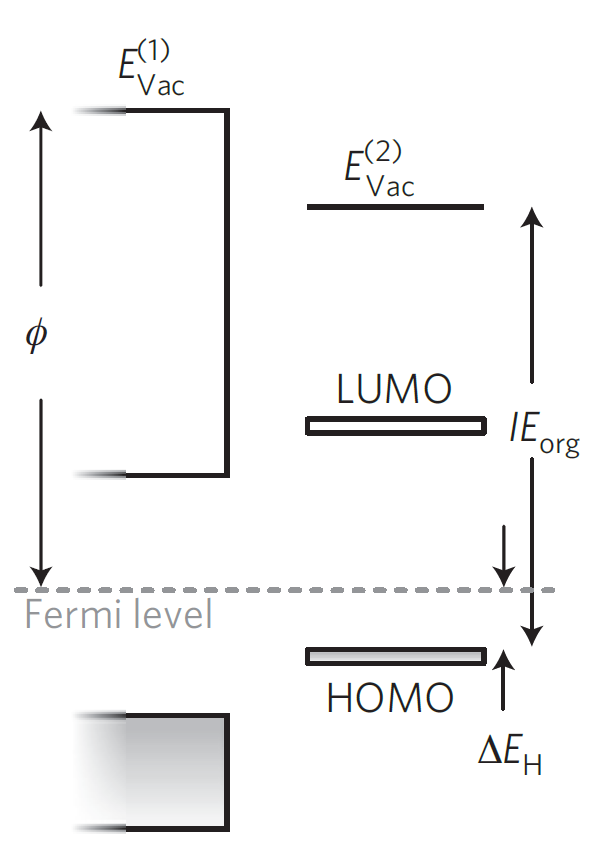
\includegraphics[height=5cm]{E_align.PNG}
                \caption{Veranschaulichung des Energieniveaus für Energieniveauanpassung des Übergangsmetalloxide und Molekülen. Kopiert aus~\cite{IF_3}.}
                \label{fig:E_align}
            \end{figure}
            % \textbf{\cite{IF_3}}
            Ferner gilt das HOMO als des Moleküls Donator-Zustand und das LUMO als Akzeptor-Zustand.
            Bei den Übergangsmetalloxiden gilt das Leitungsband als Akzeptor und das Valenzband als Donator. 
            Nur wenn sich die Donor und Akzeptor der unterschiedlichen Partner stark annähern, kann ein Ladungsaustausch stattfinden.
            Dabei ist zu beachten, dass sich durch die Wechselwirkung die energetisch Lage der Molekülorbital hinsichtlich der Gasphase verschieben können.
            Diese Energieniveaus sind in \autoref{fig:E_align} dargestellt.
            Bei der Verschiebung der Bindungsenergie des HOMOs fällt auf, dass diese sich linear immer weiter einem konstanten Wert annähert, wenn die Differenz zwischen Austrittsarbeit und Ionisationsenergie schrumpft.
            Somit wird das HOMO mit einer gewissen Bindungsenergie an das Fermilevel angeheftet, die nur von der Differenz der Austrittsarbeit und des Ionisationspotential abhängt.
            Der ganze Prozess der Ausrichtung der Molekülzustände an das Ferminiveau des Substrates wird auch Ferminiveau-Anheftung genannt~\cite{IF_3}.

            Weiter gehend ist zu beachten, dass auch bei Isolatoren sich ein Oberflächendipol ausbilden kann.
            Wegen des Pauliverbot und den zusätzlichen Elektronen der Moleküle an der Grenzfläche werden die Elektronen an der Oberfläche in den Festkörper zurück gedrenkt.
            Durch die Unabhängigkeit vom Adsorptionstyp tritt dieser \textit{Push-Back}-Effekt immer auf~\cite{IF_4} und reduziert damit das Oberflächendipolmoment~\cite{IF_1}.
            Zusätzlich kann das Oberflächendipolmoment durch Ladungsaustausch zwischen Molekül und Substrat geschwächt oder andersherum gestärkt werden.
            Hinzukommend gibt es gegebenfalls noch einen permanenten Dipol des Moleküls, welcher beachtet werden muss.
            Diese Effekte beeinflussen die Austrittsarbeit des Materials und somit auch die Ferminiveau-Anheftung.
            Als Folge des Energieniveauanpassung und dem eventuellem Ladungsaustausch oder Hybridisierung kommt es zur Verkürzung der Lebenszeit der Molekülorbital.

    \section{Substrate und Molekül Eigenschaften} \label{sec:Systeme}
        Entscheidend für alle Prozesse ist die Wahl des Substrates und der verwendeten Moleküle.
        In dieser Arbeit wurden zwei unterschiedliche Substarte gewählt.
        Beide zeigen isolierende Eigenschaften und kristalliesieren in der \ce{NaCl}-Struktur.
        Die Wahl der (111)-Orientierung ist durch die vermutete höhere Reaktivität begründet und wird in \autoref{sec:NiO} behandelt.
        Um Wüstits zu erhalten wurde zunächst Magnetit als Ausgangsmaterial verwendet, dies ist in \autoref{sec:Fe3O4} genauer beschrieben.
        Die (100) orientierte Oberfläche des Wüstits wurde gewählt um eine weniger reaktive Oberfläche zu erhalten, Näheres dazu ist in \autoref{sec:FeO} zu finden.
        Ein kleines und bereits auf vielen Oberflächen selbstanordnendes Molekül ist das Pentacene.
        Dessen Eigenschaften werden in \autoref{sec:5A} dargestellt.

        \subsection{Nickeloxid} \label{sec:NiO}
            \begin{figure}
                \centering
                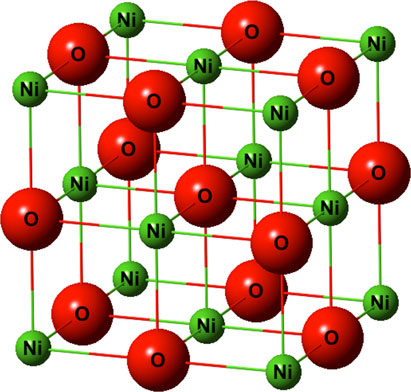
\includegraphics[height=5cm]{NiO/NiO-structure.jpg}
                \caption{Die Krsiatllstruktur von Nickeloxid. Das $\ce{Ni}^{2+}$ Ion befindet sich in einer oktaedrischen Umgebung von $\ce{O}^{2-}$ Ionen. Aus~\cite{NiO-structure}.}
                \label{fig:NiO-structure}
            \end{figure}
            Nickeloxid besitzt die Struktur von \ce{NaCl} und ist in \autoref{fig:NiO-structure} dargestellt~\cite{kunz_chemisorption_1985}.
            Hierbei handelt es sich um ein Monooxid und die Sauerstoffatome sitzen in oktaedrischen Zwischenräumen zwischen den Nickelatomen.
            Die geometrische Gitterkonstante beträgt \SI{4.17}{\angstrom}~\cite{sebbari_uranyl_2012}.
            Für die magnetische Ordnung ergibt sich die dopplte Gitterkonstante zwischen zwei gleich ausgerichteten Spins~\cite{Suter}.
            Die Austrittsarbeit lässt sich dabei durch die Präperation beeinflussen und liegt zwischen \SIrange[range-phrase=\:und\:]{4.5}{5.2}{\electronvolt}~\cite{poulain_electronic_2020}.
            % Neutronenbeugung auf Spin empfindlich also dopplte Einheitszelle, anders als die chemisch empfinliche Röntgenbeugung.

            Nickeloxid gehört zu der Familie der Antiferromagneten mit einer Neél-Temperatur von \SI{525}{\kelvin}.
            Da das 3d-Band des Nickels im Oxid nur teilweise gefüllt ist (acht von zehn möglichen Elektronen) würde erwartet werden, dass es sich hierbei um einen Leiter handelt~\cite{kunz_chemisorption_1985}.
            Dies ist allerdings nicht so und Nickeloxid ist ein Isolator, genauer ein Ladungstransfer-Isolator.
            Die Bandlücke liegt bei \SI{3.6}{\electronvolt}~\cite{kunz_chemisorption_1985}.

            Das Oberflächendipolmoment ist besonders stark in der (111)-Orientierung ausgeprägt, da bei der polaren Oberfläche entweder nur Sauerstoff oder nur Nickelionen in der obersten Lage vorhanden sind~\cite{NiO_8}.
            Dies liegt an der Bindung zwischen dem Sauerstoff und dem Nickel.
            Das Oberflächenpotential ist folglich divergent und somit die Oberfläche instabil.
            Problematisch an dünnen Filmen von Nickeloxid in der (111)-Orientierung ist diese Instabilität und die starke Abhänigkeit vom Präperationsprozess~\cite{NiO_36}.
            Es gibt verschiedene Beobachtungen zu der Stabilisierung der polaren Oberfläche wie die Rekonstruktion oder \ce{OH-}-Terminierung~\cite{NiO_36, NiO_35, NiO_34, NiO_27, NiO_10}.
            Bei der Stabilisierung wird die Oberflächenladung reduziert und damit das Oberflächenpotential gesenkt in Folge dessen es zur Ausbildung einer stabilen Oberfläche kommt.

            Die Magnetisierung ist ebenso wie die Atome abwechseln geschichtet.
            So tritt zunächst eine Ebene mit Nickel auf, in der die Magnetisierung antiparallel zu der nächsten Schicht Nickel ist.
            Die Spins innerhalb einer (111)-Ebene koppeln ferromagnetisch, wohingegen die Kopplung unter den Ebenen antiferromagnetisch ist~\cite{FeO_6}.

            Nickeloxid zeigt bereits für andere Orientierung für einige Moleküle Chemisorption, was durch enthaltene Defekt hervorgerufen wird~\cite{kunz_chemisorption_1985}.
            Auf Grund dessen eignet sich das Substrat zur Untersuchung bestens, zumal für polare Oberflächen auch eine größere Reaktivität vorhergesagt wird~\cite{cappus_hydroxyl_1993}.
            Auch die besondere Orientierung des magnetischen Moments durch die Wahl der (111)-Richtung ist bewusst gewählt, da sich so ein Schichtsystem ergibt bei dem Informationen über Spinwellen nach unten gegeben werden können.
            Besonders die hohe Geschwindigkeit der Magnonen (\si{\tera\hertz}) ist in antiferromagnetischen Materialien zu nutzen~\cite{AFM_5}.
            Hinsichtlich der elektronischen und geometrischen Struktur gibt es bereits zahlreiche Arbeiten~\cite{NiO_7, NiO_34, NiO_35, NiO_37, NiO_8, NiO_13}.
            Ferner besitzt Nickeloxid eine Gitterkonstante die ähnlich zu Gold ist, auf der sich die Moleküle wohldefiniert anordnen~\cite{5A_1}.
            
            Als zukünfiges Material in der Anwendung zeigt Nickeloxid ebenfalls bereits wichtige Eigenschaften.
            So ist Nickeloxid nicht nur ein Antiferromagnet sondern zeichnet sich auch dadurch aus, dass es die Bindungsenergie von adsorbierten Molekülen reduziert.
            Durch die geringe Bindungsenergie des HOMOs eignet sich diese Kombination dabei bestens als Lochinjektion-Material~\cite{IF_3}.
            Damit kann es in organischen Halbleitern und Bauteilen zum Einsatz kommen.

        \subsection{Magnetit} \label{sec:Fe3O4}
        \begin{figure}
            \centering
            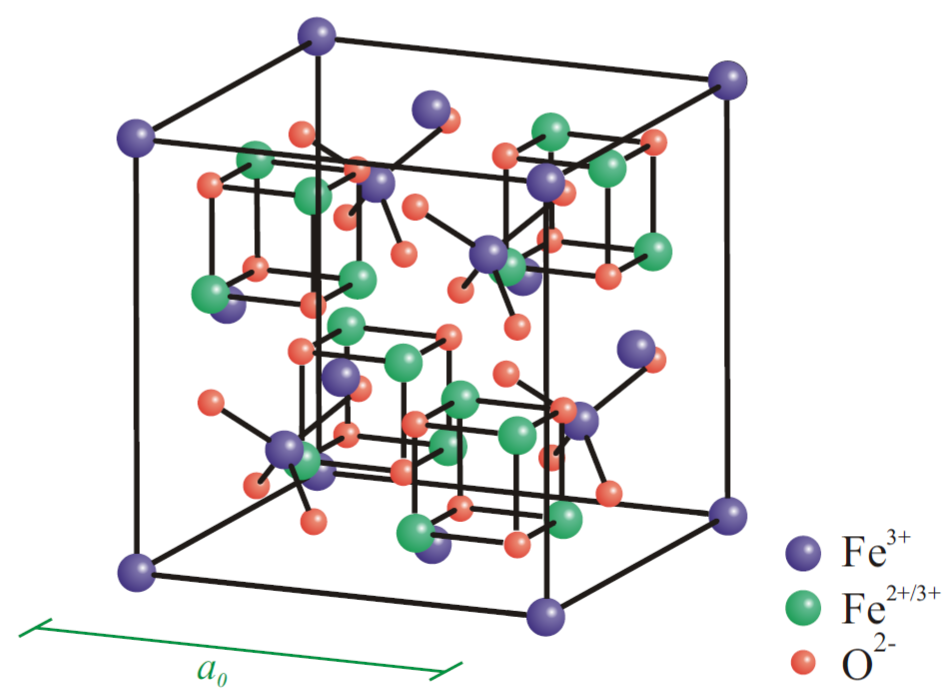
\includegraphics[height=5cm]{Spinell_mod.PNG}
            \caption{Die Krsiatllstruktur von Magnetit. Aus~\cite{bertram_rontgenstrukturanalyse_2009}.}
            \label{fig:Spinell}
        \end{figure}
            Das wohl älteste bekannte magnetische Material ist das Magnetit.
            Die Curie-Temperatur des ferrimagetischen Halbmetall Magentit liegt bei \SI{858}{\kelvin}~\cite{nordmann_anfangsstadium_2014}. % Halbmetall da ein Spinkanal isolierend der ander metallisch
            Chemisch gesehen ist es ein Eisenoxid (\ce{Fe3O4}).
            Magnetit kristallisiert in der in \autoref{fig:Spinell} dargestellten inversen Spinellstruktur, einer kubisch-flächenzentrierten Struktur.
            Die Gitterkonstante beträgt dabei \SI{8.397}{\angstrom}~\cite{springer_database}.
            Zusammen gesetzt ist das Magnetit aus zwei $\ce{Fe}^{3+}$ und einem $\ce{Fe}^{2+}$ zu vier $\ce{O}^{2-}$-Ionen.
            Hierbei befinden sich die $\ce{Fe}^{2+}$-Ionen auf $\sfrac{1}{4}$ der oktaedrischen Lücken.
            Dahingegen sitzen die $\ce{Fe}^{3+}$ zu $\sfrac{1}{4}$ auf oktaedrischen Plätzen und zu $\sfrac{1}{8}$ auf tetraedischen Plätzen.

            Die Bandlücke beträgt bei Raumtemperatur nur etwa \SI{0.1}{\electronvolt}~\cite{FeO_23}, dabei kommt ein ähnliches Prinzip des Ladungstransfer-Isolators zum Einsatz~\cite{FeO_19}.
            Durch den halbmetallischen Charakter weist Magnetit den geringsten elektrischen Widerstand aller Eisenoxide auf~\cite{FeO_23}.
            Interessanterweise unterfährt das Magnetit bei einer Temperatur von \SI{125}{\kelvin} dem Verwey Übergang und wird zum Isolator.
            Dabei ändert es nicht nur seine elektronischen Eigenschaften sondern auch die Geometrischen~\cite{cornell_iron_2003}.

            Die (100) orientierte Oberfläche hat eine $(1\times 1)\text{R}\SI{45}{\degree}$ Oberflächeneinheitszelle mit $\frac{a}{\sqrt{2}}$ Kantenlänge~\cite{bus_studies_2015}.
            Im Gegensatz zu den anderen Eisenoxiden zeigt die Oberfläche eine $(\sqrt{2}\times\sqrt{2})\text{R}\SI{45}{\degree}$ Rekonstruktion gegenüber der (100)-Orientierung des Eisens~\cite{ruwisch_vsm-untersuchung_2016}.
            Die Austrittsarbeit lässt sich dabei auf \SI{5.2}{\electronvolt} bestimmen~\cite{FeO_40}.

            Durch den Ferromagnetismus bei Raumtemperatur  ist das Material besten für die Anwendung geeignet.
            Besonders interessant wird das Material durch die \SI{100}{\percent} Spinpolarisation nahe der Fermikante.
            So lässt sich theoretisch ein unendlich großer magentischer Tunnelwiderstand erzielen~\cite{nordmann_anfangsstadium_2014}.
            Heutzutage wird Magnetit schon in Speichermedien die auf Magnetbändern fundieren eingesetzt, ebenso wie zur Katalyse~\cite{zimmermann_epitaktisches_2010}.


        \subsection{Eisenmonooxid} \label{sec:FeO}
            Ebenso wie das Nickeloxid kristallisiert auch das Eisenmonooxid, welches auch Wüstite genannt wird, in der \ce{NaCl}-Struktur~\cite{FeO_4}.
            Dabei beträgt die Gitterkonstante \SI{4.308}{\angstrom}~\cite{springer_database} und die $\ce{Fe}^{2+}$-Ionen befinden sich einer oktaedrischen Position zum Sauerstoff.
            Die $\ce{Fe}^{2+}$-Ionen bezitzen dabei sechs Elektronen im d-Niveau und bilden einen \textit{High}-Spin-Zustand.
            Fünf der sechs Spins sind also parallel ausgerichtet und der verbleibende antiparallel, was den größt möglichen Spin bewirkt~\cite{kupper_electronic_2005}.
            Allerdings ist \ce{FeO} nur oberhalb von \SI{560}{\celsius} stabil.
            Ansonsten handelt es sich um eine nichtstöchiometrische Verbindung.
            So reduziert sich der Anteil an $\ce{Fe}^{2+}$-Ionen und der Anteil an $\ce{Fe}^{3+}$-Ionen steigt~\cite{FeO_11}.
            Es sind also Defekte im Kationenteilgitter und somit wird von $\ce{Fe}_x\ce{O} (x=\num{0.95}-\num{0.88})$ gesprochen~\cite{Chalkogenide}.
            Die Verbindung kann auch in Anteile von Magnetit und Eisen übergehen.
            Dabei verändert sich dann auch die Gitterkonstante, da verschiedene Ionen unterschiedliche Bindungslängen aufweisen.

            Genau wie in Nickeloxid sind auch hier die (111)-Ebenen untereinander antiferromagnetisch gekoppelt.
            Die Neél-Temperatur liegt mit \SI{198}{\kelvin} allerdings unterhalb der Raumtemperatur~\cite{FeO_4}.
            Und die magnetischen Momente der $\ce{Fe}^{2+}$-Ionen sind parallel zu den (111)-Ebenen ausgerichtet.
            So ergibt sich auf der (100)-Oberfläche eine abwechselnde Spinausrichtung.
            Durch die Brechung der Periodizität an der Oberfläche richten sich auch die magnetischen Momente neu aus.
            In der obersten Lage nehmen diese einen Winkel von \SI{25}{\degree} mit der leichten Achse des Kristalls ([111]) hin zur Oberflächennormalen ein.
            Die inneren Lagen zeigen dabei nur noch einen Winkel zwischen \SIrange[range-phrase=\:und\:]{4}{8}{\degree} zur leichten Achse~\cite{FeO_6}.
            Als Defekte wird der Eisenmangel in oktaedrisch Umgebung und die Anreicherung von Eisenionen in tetraedischer Umgebung betrachtet.
            Steigt die Konzentration der Defekte im $\ce{Fe}_x\ce{O}$ an, so steigt ebenfalls die Neél-Temperatur an~\cite{FeO_13}.

            Wie schon das \ce{NiO} ist auch \ce{FeO} ein Ladungstransfer-Isolator mit einer Bandlücke von \SI{2.4}{\electronvolt}~\cite{FeO_21} und einer Austrittsarbeit von \SI{3.5}{\electronvolt}~\cite{FeO_28}.
            Mit dieser Energie ist eine Anregung mittels sichtbaren Lichts möglich.
            Anwendung findet dies zum Beispiel bei nanaokristallienem Eisenmonooxid als Indikator.
            Durch die antiferromagnetische Eigenschaft des Eisenmonooxid ist auch dieses für die Anwendung von optoelektrischen Bauteilen prädestiniert, da die Magnonenfrequenz im \si{\tera\hertz}-Bereich liegt.

            \begin{figure}
                \centering
                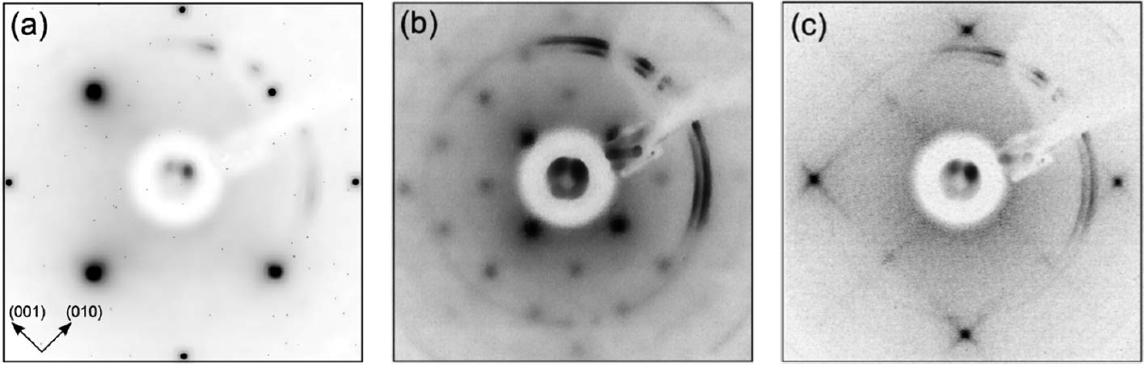
\includegraphics[height=3cm]{LEED_Sub_mod.PNG}
                \caption{Bilder der Beugung niederenergetischer Elektronen der (001)-Orientierung mit einer Elektronenenergie von \SI{125}{\electronvolt}.
                Es sind die Bilder für die passivierte Eisenoberfläche (a), den \ce{Fe3O4}-Film (b) und das Eisenmonooxid (c) gezeigt. Kopiert aus~\cite{FeO_1} und bearbeitet.}
                \label{fig:LEED_Sub}
            \end{figure}
            Die Schwierigkeit bei Eisenmonooxid besteht darin eine wohldefinierte und möglichst defektfrei Oberfläche zu erzeugen.
            Hinsichtlich dessen gab es bereits eine Vielzahl an Studien zu Kristallen des FeOs~\cite{FeO_7, FeO_19, FeO_26, FeO_23, FeO_27}, allerdings nur wenige zu der der Oberflächen~\cite{FeO_1, FeO_4, FeO_29}.
            Entscheidend für die Präperation scheint allerdings das Verhältnis aus Sauerstoffdruck und Aufdampfrate des Eisens zu sein.
            Ebenso wie die zeitliche Abfolge des Aufheizens der Probe sowie Temperaturen.
            Bei der Verwendung von passiviertem Eisen als Substrat lässt sich zunächst ein \ce{Fe3O4} Film erzeugen.
            Entsprechend ergeben sich unterschiedliche LEED-Bilder in \autoref{fig:LEED_Sub}.
            Die \ce{Fe3O4} Oberfläche zeigt dabei ein $\text{p}(2\times 2)$ Überstruktur, da die primitive Einheitszelle der Oberfläche eine Gitterkonstante von \SI{5.9}{\angstrom} besitzt.
            Damit ist sie etwa zweimal so groß wie die des passivierten Eisens mit \SI{2.86}{\angstrom}.
            Anschließend geht der Magnetitfilm in Eisenmonooxid über, wenn die Probe bei \SI{800}{\kelvin} ausgeheizt wird~\cite{FeO_1}.
            Klar ist dies an der Rekonstruktion zu erkennen, welche sich in \autoref{fig:LEED_Sub}(c) ergibt.
            Die Intensität ist dabei invertiert und die Spots sind näher zum Zentrum gerückt, auf Grund der größeren primitiven Oberflächeneinheitszelle mit $a = \SI{3.07}{\angstrom}$~\cite{FeO_1}.
            Die Reinheit kann mittels Augerelektronenspektroskopie \cite{FeO_1} oder eine genauere Identifizierung mit  Röntgenphotoelektronenspektroskopie des \ce{Fe}3p Signals erfolgen.
            Dieser enthält einen Anteil für die $\ce{Fe}^{2+}$ und $\ce{Fe}^{3+}$-Ionen~\cite{FeO_7}.


        \subsection{Pentacene} \label{sec:5A}         
            \begin{figure}
                \centering
                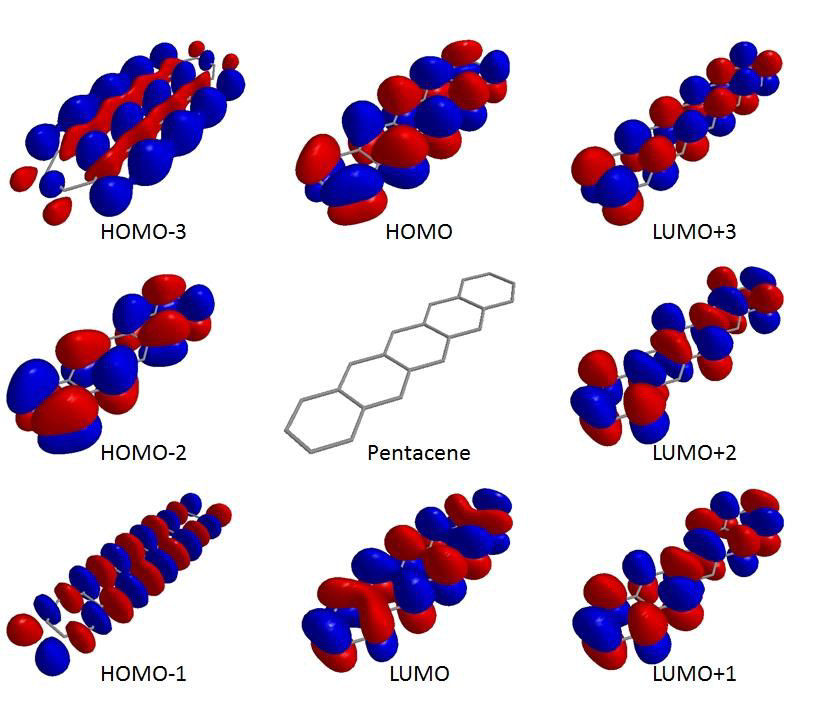
\includegraphics[width=0.6\textwidth]{PEN.jpg}
                \caption{Geometrische Struktur des Pentacene sowei die vier höchsten besetzten und vier niedrigesten unbesetzen Orbitale. Vorlage aus~\cite{PEN}.}
                \label{fig:PEN}
            \end{figure}
            Schon häufig wird Pentacene als kleines Molekül in elektronischen Bauteilen eingesetzt~\cite{5A_4}.
            Bei Pentacene ($\ce{C22H14}$) oder auch kurz 5A handelt es sich um einen Elektronendonator und gehört zu den p-Typ Halbleiter~\cite{5A_1}. % Transport wird maßgeblich durch Löcher verursacht.
            Seine Struktur ist in \autoref{fig:PEN} dargestellt, welche sich aus linear an Kanten verschmolzenen Phenylringen zusammensetzt~\cite{MM_2}.
            Ebenfalls zu sehen sind jeweils die ersten vier höchsten besetzen und niedrigsten unbesetzten Zustände.
            Pentacene bringt die perfekten Eigenschaften für Molekülorbitaltomographie mit, da es sich um ein $\pi$-konjugiertes Molekül handelt~\cite{MM_2}.
            Die Elektronen sind in den $\pi_6$-Orbitalen entlang der Phenylringen starkt delokaliert.
            Dies führt wiederum zu der bisher größten Elektronenbeweglichkeit von \SI{3.0}{\centi\meter\squared\volt\per\second} und ist sogar größer als jene des häufig eingesetzten Silizium mit \SI{1.0}{\centi\meter\squared\volt\per\second}~\cite{5A_13}.
       
            Pentacene zeigte bereits auf zahlreichen Oberflächen reproduzierbares Wachstum von dünnen Filmen bei Raumtemperatur \cite{5A_9}.
            Dabei wurden Metalle wie Gold \cite{5A_6}, Silber \cite{5A_4}, Kupfer \cite{5A_1}, Calcium \cite{5A_5} oder auch dünne Schichten aus Natriumchlorid \cite{5A_10} verwendet.
            Eine bereits häufig verwendete Oberfläche stellt die des Gold (111) dar.
            Auf ihr ordnen sich die Moleküle wohl definiert an und liegen dabei flach und parallel zum Substrat.
            Der Abstand zwischen den Molekülen und Substrat wird auf \SI{3.28}{\angstrom} bestimmt, was in der Größenordnung für Physisorption liegt~\cite{5A_1}.
            Dabei kamen Techniken wie die Rastertunnelmirkroskopie \cite{5A_7}, Beugung niederenergetischer Elektronen \cite{5A_4}, Rötgenphotoelektronenspektroskopie \cite{5A_5} sowie Molekülorbitaltomographie zum Einsatz.
            Die Molekülorbital konnten dabei zuerst mittels Rastertunnelmirkroskopie im Jahre 2011 identifiziert werden~\cite{5A_10}.

            \begin{figure}
                \centering
                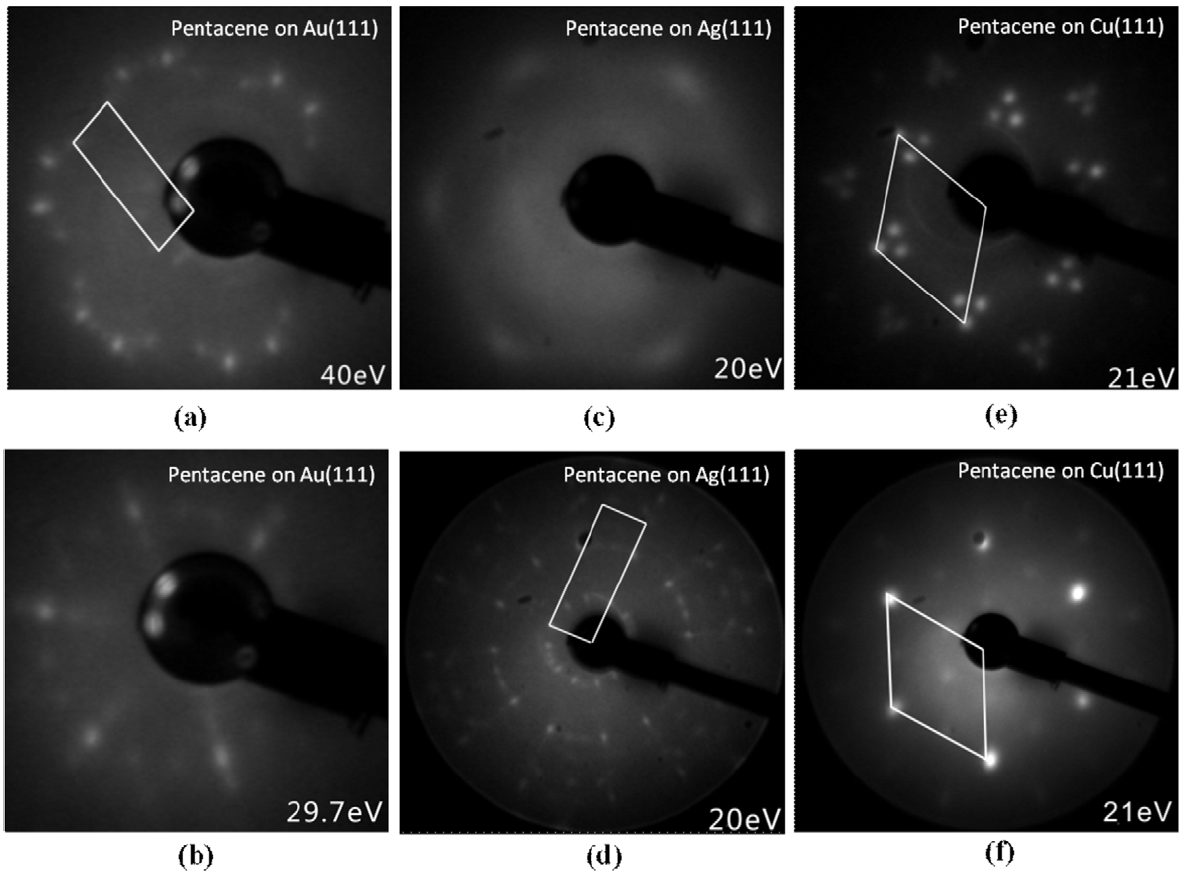
\includegraphics[width=0.6\textwidth]{PEN_Sub.PNG}
                \caption{Bilder der Beugung niederenergetischer Elektronen für verschiedene Schichtdicken und Substrate.
                Die Bilder (a), (c) und (e) entsprechen einer Bedeckung von einer Monolage, die Bilder (b), (d) und (f) einer Bilage Pentacene.
                Kopiert aus~\cite{5A_4}.}
                \label{fig:PEN_Sub}
            \end{figure}
            Dass die Wechselwirkmechanismen zwischen Substrat und Molekül eine entscheidene Rolle darstellen, lässt sich am Beispiel von Gold, Silber und Kupfer zeigen.
            Wie sich in \autoref{fig:PEN_Sub} erkennen lässt ist die Schichtdicke ebenfalls ein wichtiger Faktor bei der Selbstanordnung.
            Für die verschiedenen Substrate und Bedeckungen ergeben sich verschiedene Ordnungen auf der Oberfläche.
            Auch die Wechselwirkung reicht von Physisorption auf Au(111) über schwache Chemisorption auf Ag(111) bis hin zur starken Chemisorption auf Cu(111) \cite{5A_4}.
            Aber auch die Austrittsarbeit der Oberflächen darf bei der Untersuchung nicht ausgeschlossen werden.
            Diese zeigt einen großen Effekt auf die Ausbildung eines Oberflächendipolmoments.
            Je kleiner die Austrittsarbeit wird (je reaktiver das Substrat) desto kleiner wird auch der Oberflächendipol beim Aufbringen auf oragnischem Material \cite{5A_5}. 
            Dabei weist allerdings Pentacene keinen permanenten Dipol auf~\cite{5A_4}.

            Aktuelle Probleme sind allerdings noch die Instabilität unter Atmosphäre sowie die Löslichkeit in verschiedenen Lösungsmitteln, welche zur Massenproduktion unabdingbar ist~\cite{kus_chapter_2018}.
            Allerdings zeigten neuste Studien bereits Erfolge Pentacene aus einer Lösung als dünnen Film aufzubringen~\cite{5A_7}.
            Ein weitere großer Vorteil des Pentacene ist die einfache Herstellung \cite{kus_chapter_2018} und die Zusammensetzung aus leichten Atomen.
            Mit einer Dichte von nur \SI{1.232(6)}{\gram\per\cubic\centi\meter} ist es besonders leicht, was einen Vorteil für die mobile Anwendungen mit sich bringt~\cite{CAS}.
            
            In einigen Bauteilen kommen die Moleküle auch heutzutage schon als organischer Halbleiter zum Einsatz.
            Ausgezeichnet sind sie dafür durch die hohen Elektronenmobilität und der geringen Größe.
            Zum Bespiel in Transistoren \cite{5A_14} und Luftfeuchtigkeitssensoren \cite{demelas_chemical_2015} werden diese heute schon verwendet.
            Eine Verwendung in Solarzellen ist ebenfalls denkbar \cite{shirota_1_2019}.
            Auf Grund dessen ist eine weitere Erforschung interessant.
            So werden für den Einsatz in oragnischen Feldeffekt-Transistoren eine Schicht aus isolierendem Material, wie zum Beispiel \ce{NiO} oder \ce{FeO} und Molekülen, wie dem Pentacene benötigt~\cite{5A_13}.
            Diese Bauteile können dann in bestehende Schaltungen eingebaut werden und erhöhen so die Effizienz und können dabei die Baugröße reduzieren, sowie zur Reduktion des Gewichts beitragen.
            Versuche zur Anordnung von Pentacene auf den \ce{NiO}(111) und \ce{FeO}(100) Oberflächen konnten aktuell noch nicht beobachtet werden.
            Wohl ist aber bekannt, dass sich Pentacene auf $\ce{Fe}-\text{p}(1 \times 1)\ce{O}$ strukturiert anordnet.